\documentclass[twocolumn,10pt]{article}
\usepackage[T1]{fontenc}
\usepackage[utf8]{inputenc}
%\usepackage[english]{babel}
%\usepackage{biblatex}
\usepackage[margin=1in]{geometry}
\setlength{\columnsep}{33pt}
\setcounter{secnumdepth}{3}
\usepackage{minipage-marginpar}
\newcommand\vfilbreak[1]{\vskip 0pt plus #1 \penalty-200 \vskip 0pt plus -#1}
\newenvironment{mpmp}[1]
               {\begin{minipagewithmarginpars}{#1}}
               {\end{minipagewithmarginpars}}
\usepackage{float}
\usepackage{booktabs}
\usepackage{color}
\usepackage{graphicx}
\graphicspath{./imgs/}
\usepackage{amsmath}
\usepackage{hhline}

\title{A (failed) attempt at Lung Cancer Detection with Multi-
Instance Networks}
\author{Jay DeStories, Jason Fan, Alex Tong}

\newcommand{\red}[1]{{\color{red}#1}}
\newcommand{\temp}[1]{{\red{#1}\\}}
\renewcommand{\b}{\boldsymbol}
\newcommand\numberthis{\addtocounter{equation}{1}\tag{\theequation}}

\begin{document}
\maketitle{}

\section{Part I: The (failed) Attempt}
\subsection{Introduction and Problem Statement}
The problem of image segmentation and structure annotation within the 
field of biomedical imaging has become very active in
the past years. In 2016 and 2015, the LUng Nodule Annotation (LUNA) challenge and 
SPIE Lungx challenge, asked researchers to develop models to identify pulmonary 
nodules in lung CT slices. With the 2016 LUNA Challenge, researchers gained access
to annotated CT slices that contained segmentation ground truths for abnormal 
nodules. 
In the 2015 SPIE less than 80 CT annotated images of malignant nodules were 
released to the public.

Finally, with the 2017 Kaggle Data Science Bowl, a larger dataset of
1000+ lung CT images in DICOM format was finally released with cancer/no cancer 
labels. This has allowed researchers to answer a deeper question about lung CT
scans; whether or not there are indicators of malignancy and cancer in a patient's
CT scan.

There is, however, one caveat to the Kaggle dataset. 
Although the presence of malignancy is indicated by global, binary 
cancer/no-cancer label, the location of malignant nodules and structures are
\textit{not} annotated in the training data.

Inspired by recent work in multiple instance learning for 
whole mammogram classification
\cite{DBLP:journals/corr/ZhuLVX16},
We investigated two methods for Lung Cancer detection using Multi-Instance 
Networks.

\subsection{Related Work}
Over the past decade there has been a significant amount of work towards 
computer aided diagnosis of lung cancer \cite{cad_1998}. Depending on what kind
of data researchers have had access to, previous efforts to identify lung cancer
can be categorized by two main approaches. 
\begin{enumerate}


\item Pulmonary Nodule Detection methods. 

These methods use 
image processing techniques to segment and annotate nodules
\cite{FeatureBasedLungNoduleDetection_2017, 
     LungNoduleDetectionWeaklyLabeled_2016, U-net_2015}. These methods
mimic radiologists by looking for abnormalities in the form of
``solitary white nodule-like blob[s]" in a chest x-rays and CT scans.
Lung nodules are potential cancer indicators, and as such are an important part 
in early lung cancer diagnosis. However, not all pulmonary nodules are malignant
and many are benign, there will be false positives in diagnosis if we naively
associate nodule presence with cancer. 

\item Direct classification methods. 

These methods instead attempt to directly predict the probability of cancer using x-ray and
CT images without nodule detection.
\cite{Kuruvilla_2013, classificationOfNodules_2016}. 
\end{enumerate}
One challenge that almost all researchers in biomedical image inference face is 
small and weakly labeled datasets. Images labeled with
cancer/no-cancer binaries are weakly labeled because imaged tissues only display
malignancy locally; not \textit{all} of the tissue in an image will have cancer.
Zhu et al. in late 2016 trained a Multi-instance network on Mammogram images,
successfully demonstrating the ability for the receptive fields of a pretrained 
network to be used as instances in a biomedical image application. We take inspiration
from this paper and apply it to the 3d lung cancer case \cite{DBLP:journals/corr/ZhuLVX16, Maron:1998:FML:302528.302753}. 
% Weird that this is here... 

\subsection{Data}

The Multi-Instance Network investigated in this project are trained only on the
CT scans of 1397 patients released with the 2017 Kaggle Data Science Bowl. Each 
CT scan is a set of CT slices in the XY plane taken at different in the Z axis
(the Z axis runs parallel to the spine). The number of slices in the Z axis 
for each CT scan ranged between \red{M} and \red{N} slices.

For each CT scan, each CT slice in the XY plane is a 512 by 512 image in which
every pixel measures tissue density of a point in the thoracic cavity. Here,
density is measured by Hounsfield Units (HU), a linear scale that, unlike 
pixel values for natural images, has no upper and lower bound.
\begin{figure}[H]
\begin{center}
\label{hu_table}
\begin{tabular}{|c|c|}
\hline
Tissue & Relevant HU \\ \hhline{|=|=|}
Air & -1000 \\ \hline
Lung & $\approx -500$ \\ \hline
White/Grey Matter & 20-45 \\ \hline
Muscle & 35 - 55 \\ \hline
Bone & 700 - 3000\\ \hline
\end{tabular}
\end{center}
\caption{Respective densities of tissue}
\end{figure}
For reference respective HU values for different kinds of tissue are recorded in
Figure 1.



\subsection{Method}

We attempted to tackle this problem using Multiple Instance Learning. Multiple instance learning is a for of semi-supervised or weakly supervised learning. Instead of labels for every instance, we have labels over bags of instances that simply state whether a given class is present. In our case this means that once we have a notion of an instance of lung cancer than this will give us a way to train on more specific parts of the network. Instead of considering the entire lung for each classification, we can focus on more specific portions of the lung and thereby train faster with less overall noise.

When a radiologist examines a lung they examine nodules (small irregular tissue pieces) for potential malignancy. Each nodule can then be classified as malignant or non-malignant. In the case of lungs most nodules are non-malignant.

We would like to build in our prior knowledge about lung cancer (that nodules are useful for detection) into our model. We provide this prior as a form of MIL. Ideally, we would like to classify a lung based on all instances of nodules in a lung. If there were many nodules that are likely malignant then the whole lung should be considered cancerous. The trick is in how to get nodule instances from the lung. We thought about attempting to train a separate segmentation or object detection network to detect the nodules within the lung, but our dataset does not lend itself to that sort of detector.

We therefore use a form of receptive field MIL applied to mammogram images used by Zhu et a. \cite{DBLP:journals/corr/ZhuLVX16}. Since there are possibly many nodules in a single slice we use the receptive fields of a pretrained network as instances in our network, the idea being that a pretrained classification network such as AlexNet will have receptive fields that focus on interesting objects. Hopefully, this sort of MIL will be able to use the context around each nodule to classify malignancy. This might in an ideal lead to an out performance of human expert radiologists by considering the context around nodules instead of just the nodules themselves. 

Notice that using the receptive fields is more noisy than using more specific instances as we have to learn about what makes a malignant or non malignant receptive field, and many receptive fields may be uninteresting, providing more noise to our classification.

\subsubsection{Network Architectures}

The output of AlexNet's conv5 layer is a 256x6x6 tensor (Channels, Width Height). We perform
AlexNet on each slice leaving us with a 256x60x6x6 tensor. Each network varient then has a single learned layer on top of these features. 

We tested three network architectures on the lung volumes. A fully connected layer (FC), a Receptive Field MIL network (RF), utilizing each of AlexNets 6x6 receptive field outputs as instances, and a depth MIL network (Z), which took each slice as an instance in our multi-instance learner. 

The fully connected network is implemented as a 3D convolution of dimensions 60x6x6. This leaves us with a single value input to the sigmoid function. This is the simplest possible implementation built off of AlexNet.

We wanted to test using the receptive fields of AlexNet as MIL instances. in RF-MIL we therefore have 60x6x6 instances to learn on per image. We take a max over all instances to classify the whole lung volume.

We also wanted to compare the receptive field variant to a more standard MIL approach. in the Z-MIL network we used each of the 60 z layers as an MIL instance. This leaves us with a more reasonable number of instances to learn on.  

\begin{figure}[H]
  \label{fig:architecture}
  \begin{center}
    \begin{tabular}{ | c |c| c| }
    \hline
     FC & RF-MIL & Z-MIL\\
    \hhline{|=|=|=|}
    AlexNet\_conv5 & AlexNet\_conv5  & AlexNet\_conv5 \\
    \hline
    {conv\_(60, 6, 6)} & conv\_(1, 1, 1)  & conv\_(1, 6, 6)   \\
    \hline
    - & pool\_(60, 6, 6) & pool\_(60, 1, 1) \\
    \hline
    Sigmoid & Sigmoid & Sigmoid \\
    \hline
    \end{tabular}   
  \end{center}
  \caption{Network Architectures: conv\_(D, H, W) }
\end{figure}

\subsubsection{Pre-processing}{}

The original lung images were in DICOM format, a standard format for medical images. These files have a lot of additional meta-data about the image. We wanted to shrink and normalize the lungs as much as possible so that our system could better pick up on the important features. Since we know that radiologists when analyzing lung images for cancer look for nodules, we wanted to preserve nodules and the context surrounding them in our pre-processing. The lungs are originally 512x512 images for each slice with a variable number of slices per lung. We therefore pre-processed with the following steps. (1) For each lung slice we picked the bottom right pixel as background, and found all pixels connected of the same intensity. (2) We segmented the largest non-zero connected region as the lung volume and removed air pockets within the lung as background. (3) We scaled all pixel intensities to between zero and one, clipping at -1500, and 400. We experimented with different ways in doing this (making the mean and variance of intensity values the same as imagenet for instance), but simple scaling seemed to work best. Clipping the at these values meant that we considered a wide variaty of lung densities but ignored air and bone volumes. (4) We trimmed the edges of the lung, normalizing the scale of the lung in our image. Note that this was done in a 3d sense, so not all slices fill the entire volume. (5) We scaled the image to have dimensions 60x227x227 (Depth, Height Width). We fixed the depth to fix the z axis scale as different CT scans had a different level of Z-axis granularity.

These steps left us with a dataset of lungs with a reasonable number of slices that could be input to existing networks trained on imagenet, with also a depth axis that was approximately to scale with the real world, with each pixel representing approximately a 2mm x 2mm x 2mm volume. 


\begin{figure}[H]
\label{hounsfield_imgs}
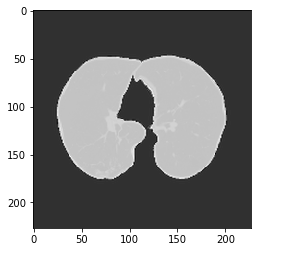
\includegraphics[width=10.9em]{imgs/hounsfield_cancer.png}
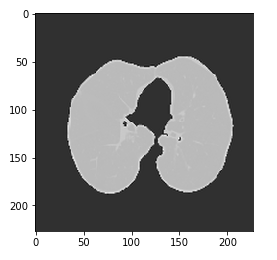
\includegraphics[width=10.7em]{imgs/hounsfield_nocancer.png}
\caption{30th slices of two lung volumes after Otsu's segmentation.
left: cancer, right: no cancer}
\end{figure}

\begin{figure*}
\label{histograms}
\begin{center}
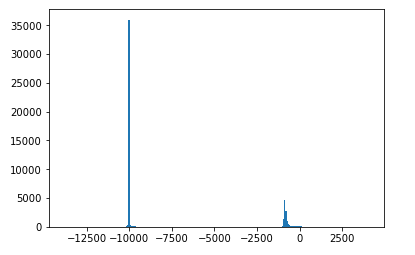
\includegraphics[width=20em]{imgs/hounsfield_hist.png}
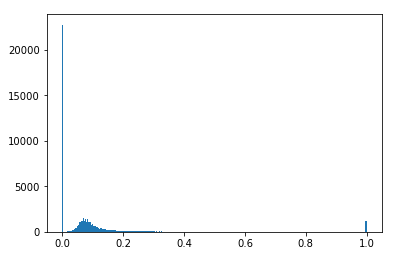
\includegraphics[width=20em]{imgs/visual_crop_hist.png}
\end{center}
\caption{Histograms of pixel intensities. Left: Hounsfield Units (HU) of 30th slice of
a lung volume after otsu's segmentation; parts of image on the perimeter outside
of the CT scan have value -10000HU. Right: pixel intensities after normalization 
and clipping of HU values with bounds -1000 and 400}
\end{figure*}

\begin{figure}[H]
\label{preprocessed_imgs}
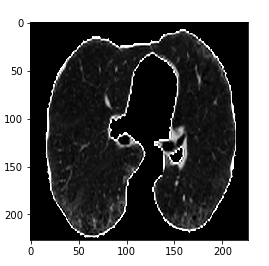
\includegraphics[width=10.8em]{imgs/visual_crop_cancer.png}
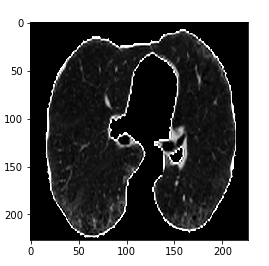
\includegraphics[width=10.8em]{imgs/visual_crop_cancer.png}
\caption{30th slices of two lung volumes after Otsu's segmentation
and pre-processing. left: cancer, right: no cancer}
\end{figure}

\subsubsection{RGB to Grayscale}
To extract features from one channel deep slices, our implementations needed to
either change the channel depth of the input or alter the first convolutional
layer of our pretrained networks.

When we attempted to use the same technique Zhu et. al. 
  used to extract slice-wise features for lung 
  volumes with pretrained convolutional neural networks (CNN),
  the networks could not fit all sixty DICOM slices of a lung volume
  into VRAM \cite{DBLP:journals/corr/ZhuLVX16}. 
  The models ran out of VRAM because, in order to use typical CNNs that 
  expect a 3 channel deep RGB image, the implementation used by Zhu et al. 
  effectively tripled the necessary data volume consumed by the first layer because it
  naively and redundantly copies each grayscale 227 by 227 slice to each of the channels;
  However, these redundant copies of the
  grayscale slices in the RGB channels can be eliminated by manipulating the first convolutional
  layer of our pretrained CNNs. 
  Let us consider the first convolution applied to one RGB pixel $\b x$,  with weight vector $\b w$, 
  bias term $b$, and test time channel-wise mean $\b \mu$. 
  If all three
  entries in $\b x$ have value $\hat x$ then,
  \begin{align*}
& \ \b w \ast (\b x - \b \mu) + b \\
= & \ (\b w \ast \b x) + (b - \b w \ast \b \mu)\\
= & \ \hat x \|\b w\|_1 + (b - \b w \ast \b \mu).
\numberthis
\end{align*}
  This means that, with weight vector $\|\b w\|_1$, bias term $(b - \b w \ast \b \mu)$ 
  and no test-time mean, a redundant 3 channel deep convolution on a
  grayscale image copied 3 times into the RGB space, can be converted
   to a 1 channel deep convolution!
  Using this RGB to grayscale conversion, our models reduced the VRAM usage in the
  first layer by a factor of 3 and could forward pass entire
  lung volumes to extract slice-wise features.



\subsubsection{Multi-Instance Learning}
In a malignant lung volume, only a small percentage of the actual tissue is
 malignant.  As such, it may not be appropriate to learn a cancer/no-cancer
 binary classification for an entire lung volume. To better model the
 sparsity of malignant tissue in a lung volume, our models instead learn a 
 cancer/no-cancer classification for patches of the lung volume.

\subsubsection{Prediction for Multi-Instance Networks}

The multiple instance models deem a lung volume cancerous if there exists
a patch that is classified to be cancerous.

Let $F$ be a set of $N$ feature vectors that each encode a patch of the Lung
CT volume. In the Z-MIL network, $F$ is a set of 60 feature vectors where
each vector is the flattened 256 by 6 by 6 output from AlexNet\_conv5. In the
RF-MIL network, $F$ is a $60 \times 6 \times 6$ set of 256 channel deep vectors.

Then, $\b r$ the vector of patchwise probabilities, is defined element wise by
\begin{equation}
r_i = \sigma(\b w^T \b f_i + b).
\end{equation}
Where $\b f_i$ and $r_i$ is the $i$-th element of $F$, and $\b r$ respectively.

We then use $\b r $ to predict the probability of cancer $p(y = 1)$ where
\begin{equation}
t = p(y = 1) = \max_{i} \ r_i.
\end{equation}

\subsubsection{Loss functions}
For the FC models, we use regular binary cross entropy loss, which is defined by,
\begin{equation}
L_{max} = -y\log(t) - (1-y)\log(1-t).
\end{equation}

For our Multi-Instance models, Z-MIL and RF-MIL, we use a loss function 
as suggested by Zhu et. al \cite{DBLP:journals/corr/ZhuLVX16}, sparse binary cross
entropy loss, that encodes the
prior belief that indicators of cancer are sparse.

\begin{equation}L_{sparse} = -y\log(t) - (1-y)\log(1-t)+ \lambda_r\|\b r\|_1
\end{equation}
Here the regularizing parameter $\lambda_r\|\b r\|_1$ is scaled by
hyperparameter $\lambda_r$.

Sparse binary cross entropy loss penalizes a model that classify many instances 
to be cancerous. It encourages the model to only classify
few instances to be cancerous which better models our understanding of 
cancer.

\subsubsection{Augmentation}

Initial experiments showed that, because of the small data volume, every models 
easily overfit to either training set; each achieved almost 0 training loss within
100 epochs without significant decrease in validation loss.
 To prevent overfitting, at training time, each mini-batch is augmented. Each
mini-batch is randomly shifted in the Z axis by 0 to 10 voxels, in the X axis by 
0 to 50 pixels and also in the Y axis by 0 to 50 pixels. Each mini-batch is then
also randomly flipped with probability \(\frac 1 2\).

This stopped our models from reaching perfect training loss and overfitting.

\subsubsection{Training}

Initial experiments with the training data, the models were easily confused and 
predicted class probabilities probabilities equal to the proportion of cancerous
lungs to total lungs. Because of this, some models were trained on a subset of 
the entire training set in which the number of cancer and no cancer samples
were equal.
\begin{figure}[H]
  \label{fig:data_distributions}
  \begin{center}
    \begin{tabular}{ | c || c |c| c| }
    \hline
     - & Unbalanced & Balanced & Test\\
    \hhline{|=||=|=|=|}
    \# Cancer & 362 & 322 & 50 \\
    \hline
    \# No Cancer & 1035 & 322 & 121\\
    \hline
    \# Total & 1397 & 644 & 171\\
    \hline
    \end{tabular}  
\end{center}
    \caption{Class distributions for datasets}
\end{figure}

We used ADAM with default parameters and experimented with the Initial learning rate, the learning rate decay and the number of epochs. Training was done both on a GTX 1080 Ti and a K80 Amazon instance GPU. We found that the 1080 Ti was up to 3x faster than the K80 in training.

\begin{figure}[H]
\label{lung_results}
\begin{center}
\newcommand{\e}{\mbox{e}}
\begin{tabular}{|c|c|c|c|c|}
\hline 
Model & Dataset & Initial LR& Decay& Epochs \\
\hline
FC & unbalanced &  $1\e^{-5}$ & 0.85 & 200 \\
Z-MIL & balanced & $1\e^{-5}$ & 0.95 & 500 \\
Z-MIL & unbalanced &  $1\e^{-5}$ & 0.95 & 200 \\
FC & balanced & $1\e^{-5}$ & 0.85  & 200 \\
RF-MIL & balanced & $4\e^{-3}$ & 1.00 & 500 \\ %OH NO!
\hline
\end{tabular}
\end{center}
\caption{Training hyperparameters for respective models}
\end{figure}




\subsection{Results}

We report the best test set loss and average precision for all three networks. The RF-MIL network was not able to train on the unbalanced dataset. While the RF-MIL network had the lowest loss cross-entropy loss of all three networks on the balanced dataset, it also had the lowest average precision. We suspect that this implies not that the RF-MIL network performed the best, but that the cross entropy loss is a poor measure for this data. Overall we see that the FC network had the best performance as measured by AP. 

\begin{figure}[H]
\label{lung_results}
\begin{center}
\begin{tabular}{|c|c|c|c|}
\hline 
Model & Dataset & Loss& AP \\
\hline
FC & unbalanced &  0.621 & 0.407 \\ %200
Z-MIL & balanced & 0.783 & 0.399 \\ % 500
Z-MIL & unbalanced &  0.684 & 0.346 \\ %200
FC & Balanced & 0.865 & 0.302 \\ %200
RF-MIL & Balanced & 0.720 & 0.293 \\ %500
\hline
\end{tabular}
\end{center}
\caption{Results for Lung Cancer Detection}
\end{figure}

\begin{figure*}
\label{lung_pr_curves}
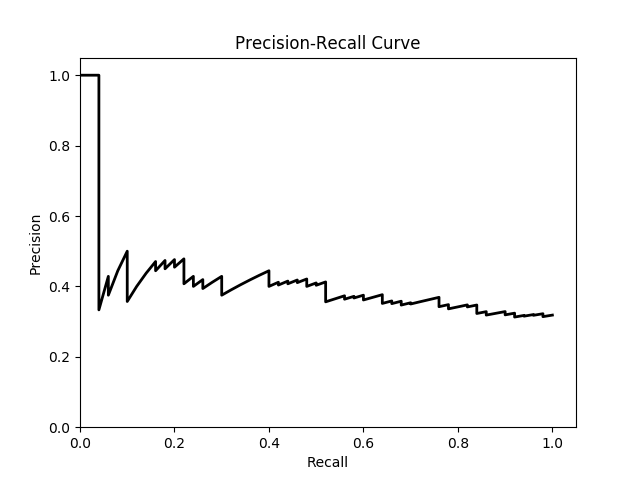
\includegraphics[width=15em]{imgs/alexslicerunbalancednotrim_pr.png}
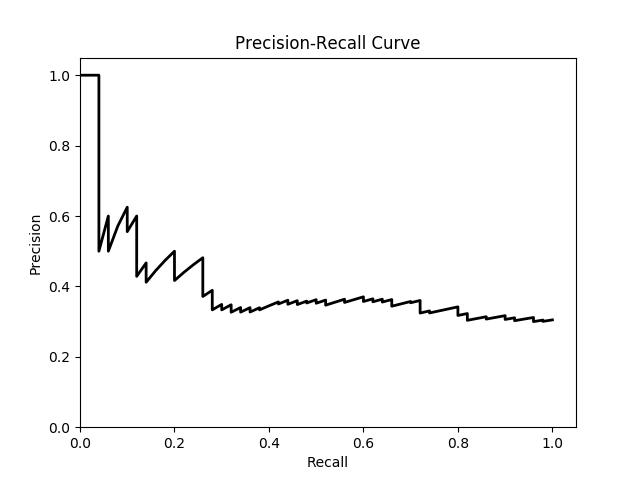
\includegraphics[width=15em]{imgs/alexslicerZMIL_pr.png}
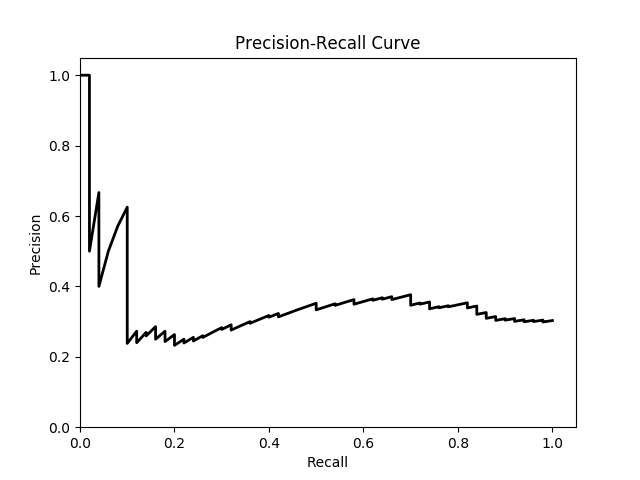
\includegraphics[width=15em]{imgs/alexslicerZMILunbalancednotrim_pr.png}
\caption{Precision recall curves for the following three models. From left to
right: FC trained on unbalanced, Z-MIL trained on balanced, Z-MIL trained on
unbalanced.}
\end{figure*}

\section{Part II: Why did the networks fail?}

Our networks built on top of pretrained AlexNet failed to learn anything useful from the data. We now examine the possible reasons why this was so. 

\subsection{A second look at the data}

The Lung Image Data Consortium image collection (LIDC), is a similar dataset to the one Kaggle published, however it includes additional nodule level tags such as location, diameter, and malignancy. The top Kaggle submissions did not train on the provided Kaggle data, and trained on LIDC data instead. This is due to a ``loophole" in the Kaggle challenge rules that all any publicly available data to be used as additional training data. This additional data allowed them to use nodule level tags to improve their training. This is a clear advantage over the Kaggle dataset where we are not able to eliminate other lung noise as easily. 

The lungs are approximately 400x400x400mm in scale where the average diameter of a nodule in the LIDC dataset is 4.8mm. This means that the signal to noise ratio (if we only consider nodules as signal) is 1,000,000:1. With the given dataset size, even with augmentation, we do not have nearly enough data to learn this signal. LIDC data would have allowed training on a more reasonable signal to noise ratio. When we downsample to 60x227x227 this means that a nodule will be approximately 1x3x3 pixels. This is probably too small to get any meaningful data about whether that nodule is malignant or not. We suspect training on the full data might have prevented this problem or at least minimized its effect.


\subsection{HOG features + SVM baseline}

We attempted to set a baseline with slicewise HOG features with PCA fed into a support vector machine. The results in Figure 10 show that we were not able to do any better than random. We suspect this has to do with the relative size of the nodules and the number of hog features that are uninformative. 

We trained on the Balanced dataset which had 644 lungs in the training set (hence the maximum kernal size of 644. Augmentation was not performed during training. Most parameter settings resulted in the SVM predicting all lungs as non-cancerous. This results in a 70.7\% accuracy on our test set as the proportion of non-cancerous lungs. 

\begin{figure}[H]
\label{svm_result}
\begin{center}
\begin{tabular}{|c|c|c|c|c|c|}
\hline
Kernel & Dim. & SVM Loss & Acc. & Prec. & Rec. \\ \hline
RBF* &  32 & 0.60 & 0.707 & 0 & 0 \\ 
RBF* & 644 & 0.75 & 0.707 & 0 & 0 \\
Lin. & 64 & 0.61 & 0.713 & 0.57 & 0.08 \\
Lin. & 644 & 1.00 & 0.631 & 0.24 & 0.12 \\
Sigmoid.* & 644 & 0.778 & 0.707 & 0 & 0 \\
\hline
\end{tabular}
\end{center}
\caption{Results from HOG-SVM experiments}
\end{figure}

\subsection{Testing RF-MIL}

We wanted to investigate our RF-MIL network on different easier to work with data. So we compared it's performance to the FC network on a constructed dataset built off of the ants and bees pytorch example. 

\begin{figure*}
\label{ants_bees_imgs}
\begin{center}
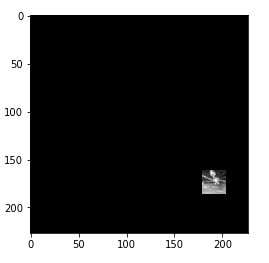
\includegraphics[width=11em]{imgs/ant1.png}
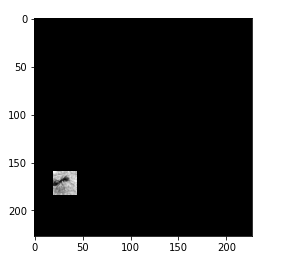
\includegraphics[width=11.5em]{imgs/ant2.png}
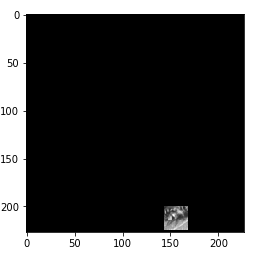
\includegraphics[width=10.8em]{imgs/bee1.png}
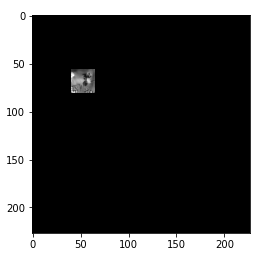
\includegraphics[width=11.1em]{imgs/bee2.png}
\end{center}
\caption{Example of randomly embeded 25 by 25 images of ants and bees. 
From left to right, the classes are: ant, ant, bee, bee.}
\end{figure*}
\subsubsection{Architectures}

\begin{figure}[H]
  \label{fig:ab_architecture}
  \begin{center}
    \begin{tabular}{ | c |c|}
    \hline
     FC & RF-MIL\\
     \hhline{|=|=|}
    AlexNet Conv5 & AlexNet Conv5 \\
    \hline
    {Conv2D  (6, 6)} & Conv2D (1, 1) \\
    \hline
    - & Pool (6,6) \\
    \hline
    Sigmoid & Sigmoid \\
    \hline
    \end{tabular}   
  \end{center}
  \caption{Network Architectures for Toy Example}
\end{figure}

\subsubsection{Toy Data}
We generated best case, toy datasets that model low signal strength
and also low noise inputs by embedding grayscale images of Ants and Bees onto a
black background (shown in Figure 11). We wanted to ask the question how small a signal can the MIL network detect? Therefore we altered the sizes and random placement of the ant/bee images in a black background and measured the results. 

\subsubsection{Training}
\begin{figure}[H]
\label{ab_training}
\begin{center}
\newcommand{\e}{\mbox{e}}
\begin{tabular}{|c|c|c|c|c|}
\hline 
Model  & Initial LR& Decay& Epochs \\
\hline
FC  &  $1\e^{-3}$ & 0.95 & 50 \\
MIL  & $2\e^{-3}$ & 0.85 & 50 \\
\hline
\end{tabular}
\end{center}
\caption{Training hyperparameters for ants and bees models}
\end{figure}

We again used ADAM for backpropogation. We tried a couple of different hyperparemter settings for the ants and bees model shown in Figure 13. 

\subsubsection{Results}

The FC network outperformed our RF-MIL network. We hypothesis that the RF-MIL network would work best in the case where the image was full of bees and a single randomly placed ant image and asked the question is there an ant in this image? We suspect the fully connected network would classify the image as bees only as it would not have the 36 separate instance evaluations that the RF-MIL network has. 
\begin{figure}[H]
  \label{fig:architecture}
  \begin{center}
    \begin{tabular}{ |c|c|c|c|c|}
    \hline
    Model & Random XY & Size & Loss & AP \\\hhline{|=|=|=|=|=|}
MIL  & N/A & 227 & 0.451 & 0.896 \\ \hline
FC & N/A & 227 & 0.585 & 0.898 \\ \hline
MIL & False & 113 & 0.610 & 0.753\\ \hline
FC & False & 113 & 0.480 & 0.873\\ \hline
MIL & True & 113 & 0.569 & 0.804\\ \hline
FC & True &113 &0.466 &0.871\\ \hline
MIL &False &50 &0.684 &0.660\\ \hline
FC &False &50 &0.558 &0.809\\ \hline
MIL &True &50 &0.673 &0.703\\ \hline
FC &True &50 &0.573 &0.782\\ \hline
MIL &False &25 &0.687 &0.631\\ \hline
FC &False &25 &0.611 &0.742\\ \hline
MIL &True &25 &0.652 &0.709\\ \hline
FC &True &25 &0.605 &0.767\\\hline
MIL &False &5 &0.692* &0.582\\\hline
FC &False &5 &0.688 &0.576\\\hline
MIL &True &5 &0.686 &0.588\\\hline
FC &True &5 &0.681 &0.581\\ \hline
    \end{tabular}   
  \end{center}
  \caption{Results from Ants vs. Bees Classification Test. Size - the height and
  width of the embedded image in the 227 by 227 input. Random XY - whether or not
  the embedded image was embedded in a random location; if false, embedded image
  was embedded in the top left hand corner.}
\end{figure}

\section{Part III: Conclusions and lessons learned}

In conclusion we learned that Multiple Instance Learning is not as easy as it seems. The data bottleneck placed by performing a max over all instances limits the rate at which the network is able to learn. Since only one instance is updated by backpropogation per time step then it might potentially take \textit{\# of receptive fields} times as long to train the network. We would like to try other MIL methods for final classification (not a simple max) such as a weighted ranking of instances. This would allow the gradient to backpropogate to all instances during each training timestep potentially leading to a huge increase in training speed.

More generally, we were misled by the amount of data. Since each lung provides so much data, we thought we could learn something from the hundreds of gigabytes of data in total. We forgot to consider the importance of the annotations on that data. With the addition of nodule level annotations the effective size of the data explodes. Next time we approach a deep learning problem we will weigh not only the training set size but the annotation quality as well. 


\bibliographystyle{unsrt}%Used BibTeX style is unsrt
\bibliography{final}
\end{document}
